% Q4 -- CMOS pseudo-static D latch / "D flip-flop" using transmission gates.
% TEXTBOOK FORM: TWO transmission gates + TWO inverters (NOT gates).
% Forward: D -TG1(phi)-> node A -inv1-> Q.  Feedback (holds A): Q -inv2-> -TG2(phi-bar)-> A.
% phi high  : TG1 on, TG2 off -> A follows D (transparent / sample).
% phi-bar high: TG1 off, TG2 on -> 2-inverter loop holds A (pseudo-static refresh).
% NOTE: strictly this single-stage cell is a level-sensitive LATCH; the textbook
% (Pucknell) calls it a "pseudo-static D flip-flop". A true edge-triggered FF = two
% such stages (master+slave) on opposite clock phases.
\documentclass[border=10pt]{standalone}
\usepackage{tikz}
\usetikzlibrary{arrows.meta}
\begin{document}
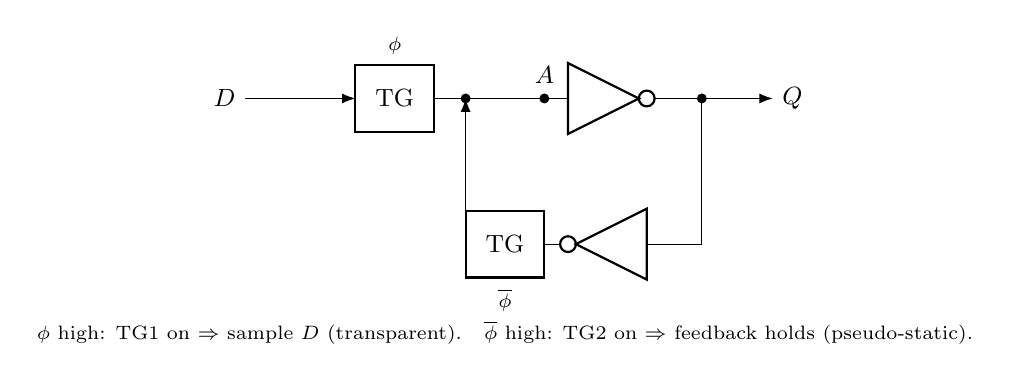
\begin{tikzpicture}[>=Latex, font=\small,
  tg/.style={draw, thick, minimum width=1.0cm, minimum height=0.85cm}]
% --- forward path: D - TG1(phi) - A - inv1 - Q ---
\draw[->] (-0.4,0) node[left]{$D$} -- (1.0,0);
\node[tg] (tg1) at (1.5,0) {TG};
\node[above, font=\scriptsize] at (tg1.north) {$\phi$};
\draw (tg1.east) -- (3.4,0) coordinate (A);
\fill (A) circle (1.8pt);  \node[above=2pt] at (A) {$A$};
% inverter 1 (forward): triangle + bubble
\draw[thick] (3.7,0.45) -- (3.7,-0.45) -- (4.6,0) -- cycle;
\draw[thick] (4.7,0) circle (0.1);
\draw (A) -- (3.7,0);
\draw[->] (4.8,0) -- (6.3,0) node[right]{$Q$};
\fill (5.4,0) circle (1.8pt);
% --- feedback path: Q - inv2 - TG2(phi-bar) - back to A ---
% inverter 2 (feedback), pointing left
\draw[thick] (4.7,-1.85+0.45) -- (4.7,-1.85-0.45) -- (3.8,-1.85) -- cycle;
\draw[thick] (3.7,-1.85) circle (0.1);
\draw (5.4,0) -- (5.4,-1.85) -- (4.7,-1.85);
\node[tg] (tg2) at (2.9,-1.85) {TG};
\node[below, font=\scriptsize] at (tg2.south) {$\overline{\phi}$};
\draw (3.6,-1.85) -- (tg2.east);
\draw[->] (tg2.west) -- (2.4,-1.85) -- (2.4,0);
\fill (2.4,0) circle (1.8pt);
\node[font=\scriptsize, align=center, anchor=north] at (2.9,-2.7)
 {$\phi$ high: TG1 on $\Rightarrow$ sample $D$ (transparent).\quad
  $\overline{\phi}$ high: TG2 on $\Rightarrow$ feedback holds (pseudo-static).};
\end{tikzpicture}
\end{document}
